\begin{itemize}
	\begin{center}
	    Paso 1
	\end{center}
	

	    Primero abrimos el Hyper-v, nos dirijimos donde dice Administrador de conmutadores virtuales hacemos click, después se abrirá otra ventana donde saldrá para crear el Conmmutador Virtual le colocamos cualquier nombre, como lo puedes observar en la siguiente imagen.
		\begin{center}
		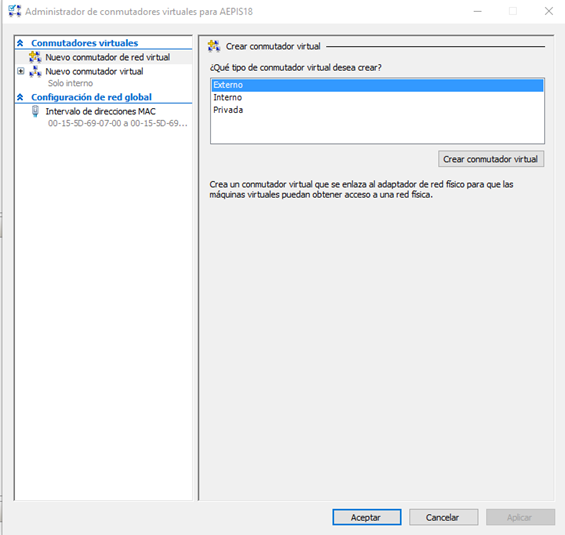
\includegraphics[width=15cm]{./Imagenes/imagen1} 
		\end{center}
	

	\end{itemize} 
	

	\begin{itemize}
	\begin{center}
	    Paso 2
	\end{center}
	

	    Despues nos dirigimos a Configuracion de hyper-v, se abrirá una ventana. 
		\begin{center}
		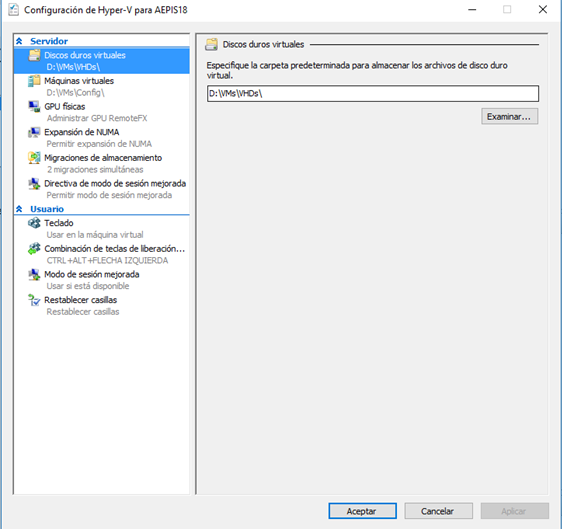
\includegraphics[width=15cm]{./Imagenes/imagen2} 
		\end{center}
	

	\end{itemize} 
	
	
	\begin{itemize}
	\begin{center}
  	  Paso 3
	\end{center}


   	 Seguidamente hacemos click en Discos Duros Virtuales\\
	\begin{center}
	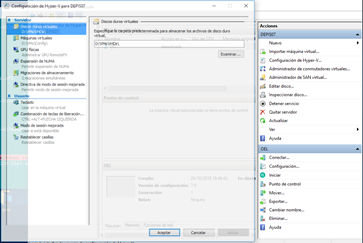
\includegraphics[width=15cm]{./Imagenes/imagen3} 
	\end{center}


	\end{itemize} 


	\begin{itemize}
	\begin{center}
 	   Paso 4
	\end{center}


   	 Luego hacemos click en examinar y agregamos la siguiente carpeta que creamos en el Disco D, con el nombre de VHDs, le damos click en Seleccionar Carpeta, como se puede observar en la imagen.\\
	\begin{center}
	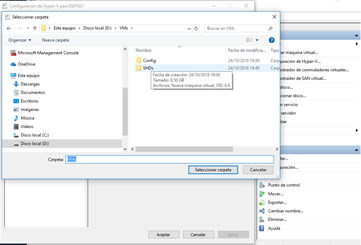
\includegraphics[width=15cm]{./Imagenes/imagen4} 
	\end{center}


	\end{itemize}
	
	\begin{itemize}
	\begin{center}
    Paso 5
	\end{center}


   Despues seleccionamos Maquinas Virtuales y le hacemos click en examinar.\\
	\begin{center}
	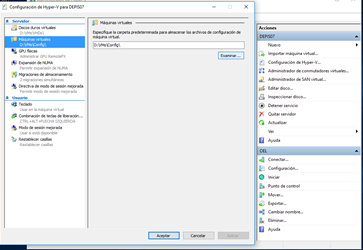
\includegraphics[width=15cm]{./Imagenes/imagen5} 
	\end{center}


	\end{itemize} 


	\begin{itemize}
	\begin{center}
   	 Paso 6
	\end{center}


 	   Continuando con el paso anterior se abrirá una ventana donde seleccionamos la siguiente carpeta con el nombre de Config, le hacemos click en Selecciona Carpeta. Despues le damos click en Aplicar y después en aceptar. \\
	\begin{center}
	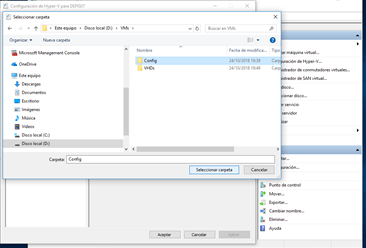
\includegraphics[width=15cm]{./Imagenes/imagen6} 
	\end{center}


	\end{itemize} 
	\begin{itemize}
\begin{center}
    Paso 7
\end{center}


    En este paso, crearemos una Maquina Virtual, le damos click en Nuevo-Maquina Virtual \\
	\begin{center}
	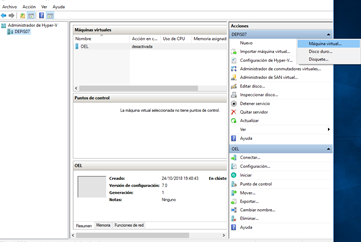
\includegraphics[width=15cm]{./Imagenes/imagen7} 
	\end{center}


\end{itemize} 


\begin{itemize}
\begin{center}
    Paso 8
\end{center}


    Luego se abrirá una ventana de Asistente para crear una maquina virtual, le damos click en el botón siguiente hasta que finalice el crear la maquina virtual al cual le dimos el nombre de OEL.\\
	\begin{center}
	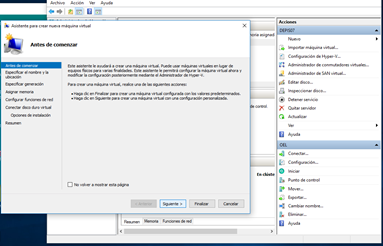
\includegraphics[width=15cm]{./Imagenes/imagen8} 
	\end{center}


\end{itemize} 



  
  
  

